\documentclass[12pt,letterpaper]{article}
\usepackage{graphicx,textcomp}
\usepackage{natbib}
\usepackage{setspace}
\usepackage{fullpage}
\usepackage{color}
\usepackage[reqno]{amsmath}
\usepackage{amsthm}
\usepackage{fancyvrb}
\usepackage{amssymb,enumerate}
\usepackage[all]{xy}
\usepackage{endnotes}
\usepackage{lscape}
\newtheorem{com}{Comment}
\usepackage{float}
\usepackage{hyperref}
\newtheorem{lem} {Lemma}
\newtheorem{prop}{Proposition}
\newtheorem{thm}{Theorem}
\newtheorem{defn}{Definition}
\newtheorem{cor}{Corollary}
\newtheorem{obs}{Observation}
\usepackage[compact]{titlesec}
\usepackage{dcolumn}
\usepackage{tikz}
\usetikzlibrary{arrows}
\usepackage{multirow}
\usepackage{xcolor}
\newcolumntype{.}{D{.}{.}{-1}}
\newcolumntype{d}[1]{D{.}{.}{#1}}
\definecolor{light-gray}{gray}{0.65}
\usepackage{url}
\usepackage{listings}
\usepackage{color}

\definecolor{codegreen}{rgb}{0,0.6,0}
\definecolor{codegray}{rgb}{0.5,0.5,0.5}
\definecolor{codepurple}{rgb}{0.58,0,0.82}
\definecolor{backcolour}{rgb}{0.95,0.95,0.92}

\lstdefinestyle{mystyle}{
	backgroundcolor=\color{backcolour},   
	commentstyle=\color{codegreen},
	keywordstyle=\color{magenta},
	numberstyle=\tiny\color{codegray},
	stringstyle=\color{codepurple},
	basicstyle=\footnotesize,
	breakatwhitespace=false,         
	breaklines=true,                 
	captionpos=b,                    
	keepspaces=true,                 
	numbers=left,                    
	numbersep=5pt,                  
	showspaces=false,                
	showstringspaces=false,
	showtabs=false,                  
	tabsize=2
}
\lstset{style=mystyle}
\newcommand{\Sref}[1]{Section~\ref{#1}}
\newtheorem{hyp}{Hypothesis}

\title{Problem Set 1}
\date{
	Name: Darragh McGee (18319331)\\
}
\author{Applied Stats/Quant Methods 1}

\begin{document}
	\maketitle

	\section*{Question 1: Education}

A school counselor was curious about the average of IQ of the students in her school and took a random sample of 25 students' IQ scores. The following is the data set:\\
\vspace{.5cm}
\lstinputlisting[language=R, firstline=40, lastline=41]{PS01_answers_DMcG.R}  
\vspace{.5cm}

\begin{enumerate}
\item \textbf{Find a 90\% confidence interval for the average student IQ in the school.}
\end{enumerate}

\noindent 90 Percent Confidence Interval = Point Estimate i.e. Mean +/- Margin of Error (Critical Value*Standard Error)

\vspace{.5cm}
\noindent\textbf{Step 1:} Input Data Set of Student IQs and Create Vector
\lstinputlisting[language=R, firstline=40, lastline=41]{PS01_answers_DMcG.R} 

\vspace{.5cm}
\noindent\textbf{Step 2:} Calculating Mean Student Height
\lstinputlisting[language=R, firstline=43, lastline=44]{PS01_answers_DMcG.R} 
Mean Student IQ =  98.44

\vspace{.5cm}
\noindent\textbf{Step 3:} Calculating Standard Error
\lstinputlisting[language=R, firstline=47, lastline=48]{PS01_answers_DMcG.R} 
Standard Error = 2.618575

\vspace{.5cm}
\noindent\textbf{Step 4:} Calculate Test Statistic for 90 Percent Confidence Level

\noindent As the sample size is 25 (Less than 30) a T-Distribution should be used for Critical Value.  

\vspace{.5cm}
\noindent T-Statistic Formula requires Degrees of Freedom Degrees of Freedom (n-1)
\lstinputlisting[language=R, firstline=56, lastline=57]{PS01_answers_DMcG.R} 

Degrees of Freedom = 24

\vspace{.5cm}
\noindent T-Statistics for 90 Percent Confidence Interval is interested in the Critical Value for the First 5 Percent and Last 5 Percent of the Distribution 
\lstinputlisting[language=R, firstline=61, lastline=64]{PS01_answers_DMcG.R} 
t-score = +/- 1.710882

\vspace{.5cm}
\noindent\textbf{Step 5: }Construct 90 Percent Confidence Interval 
\lstinputlisting[language=R, firstline=67, lastline=70]{PS01_answers_DMcG.R} 
90 Percent Confidence Interval = 93.95933 to 102.9201

\vspace{.5cm}
\noindent \textbf{Validating Approach:} Using in-built t.test() formula in R to check results
\lstinputlisting[language=R, firstline=75, lastline=75]{PS01_answers_DMcG.R}
\begin{verbatim}
	90 percent confidence interval:
	93.95993 102.92007
	sample estimates:
	mean of x 
	98.44 
\end{verbatim}
The results from the in-built t.test function are equal to the step-by-step calculations (allowing for marginal rounding differences). 

\newpage 
\begin{enumerate}
\setcounter{enumi}{1}
	\item Next, the school counselor was curious  whether  the average student IQ in her school is higher than the average IQ score (100) among all the schools in the country. 
	
	\noindent Using the same sample, conduct the appropriate hypothesis test with $\alpha=0.05$.
\end{enumerate}
\textbf{Step 1:} Assumptions about Data
\begin{itemize}
\item
Sample Size is below 30. Therefore, T-Statistic should be used.
\item 
Population IQ = 100
\item
IQ represents continuous data
\item
Random Sampling Conducted
\item
The data is approximately normally distributed. 
\item
Observations are independent of one another. 
\end{itemize}
\vspace{.5cm}
\textbf{Step 2: }Setting Up Hypothesis
\begin{itemize}
\item
\textbf{Null Hypothesis:} The average Student IQ in the sample school is less than or equal to the average IQ score (100) among all the schools in the country 
\item
\textbf{Alternative Hypothesis:} The average student IQ in the sample school is greater than the average IQ score (100) among all the schools in the country
\end{itemize}

\vspace{.5cm}
\noindent\textbf{Steps 3:} Calculate the Test-Statistic 
\lstinputlisting[language=R, firstline=94, lastline=96]{PS01_answers_DMcG.R}
T-Statistic = -0.5957439

\vspace{.5cm}
\noindent\textbf{Steps 4:} Calculate the p-value 
\lstinputlisting[language=R, firstline=99, lastline=100]{PS01_answers_DMcG.R}
p-value = 0.7215383

\vspace{.5cm}
\noindent\textbf{Step 5:} Conclusion  
\begin{itemize}
	\item 
Fail to reject the Null Hypothesis as the p-value is greater than 0.05 (exceeding the 5 percent significance level). 
\item 
There is insufficient evidence to conclude that the sample mean is greater than 100.
\end{itemize}

\newpage
	\section*{Question 2: Political Economy}

\noindent Researchers are curious about what affects the amount of money communities spend on addressing homelessness. The following variables constitute our data set about social welfare expenditures in the USA. \\

\begin{tabular}{r|l}
	\texttt{State} &\emph{50 states in US} \\
	\texttt{Y} & \emph{per capita expenditure on shelters/housing assistance in state}\\
	\texttt{X1} &\emph{per capita personal income in state} \\
	\texttt{X2} &  \emph{Number of residents per 100,000 that are "financially insecure" in state}\\
	\texttt{X3} &  \emph{Number of people per thousand residing in urban areas in state} \\
	\texttt{Region} &  \emph{1=Northeast, 2= North Central, 3= South, 4=West} \\
\end{tabular}

\vspace{.5cm}
\noindent Explore the \texttt{expenditure} data set and import data into \texttt{R}.
\vspace{.5cm}
\lstinputlisting[language=R, firstline=117, lastline=117]{PS01_answers_DMcG.R}  
\vspace{.5cm}
\begin{itemize}
\item
Please plot the relationships among \emph{Y}, \emph{X1}, \emph{X2}, and \emph{X3}? What are the correlations among them (you just need to describe the graph and the relationships among them)?
\vspace{.5cm}
\end{itemize}

\newpage
\lstinputlisting[language=R, firstline=124, lastline=127]{PS01_answers_DMcG.R}
\begin{figure}[H]
	\caption{Scatterplot of relationship between per capita expenditure on housing assistance and personal income in state}
	\centering
	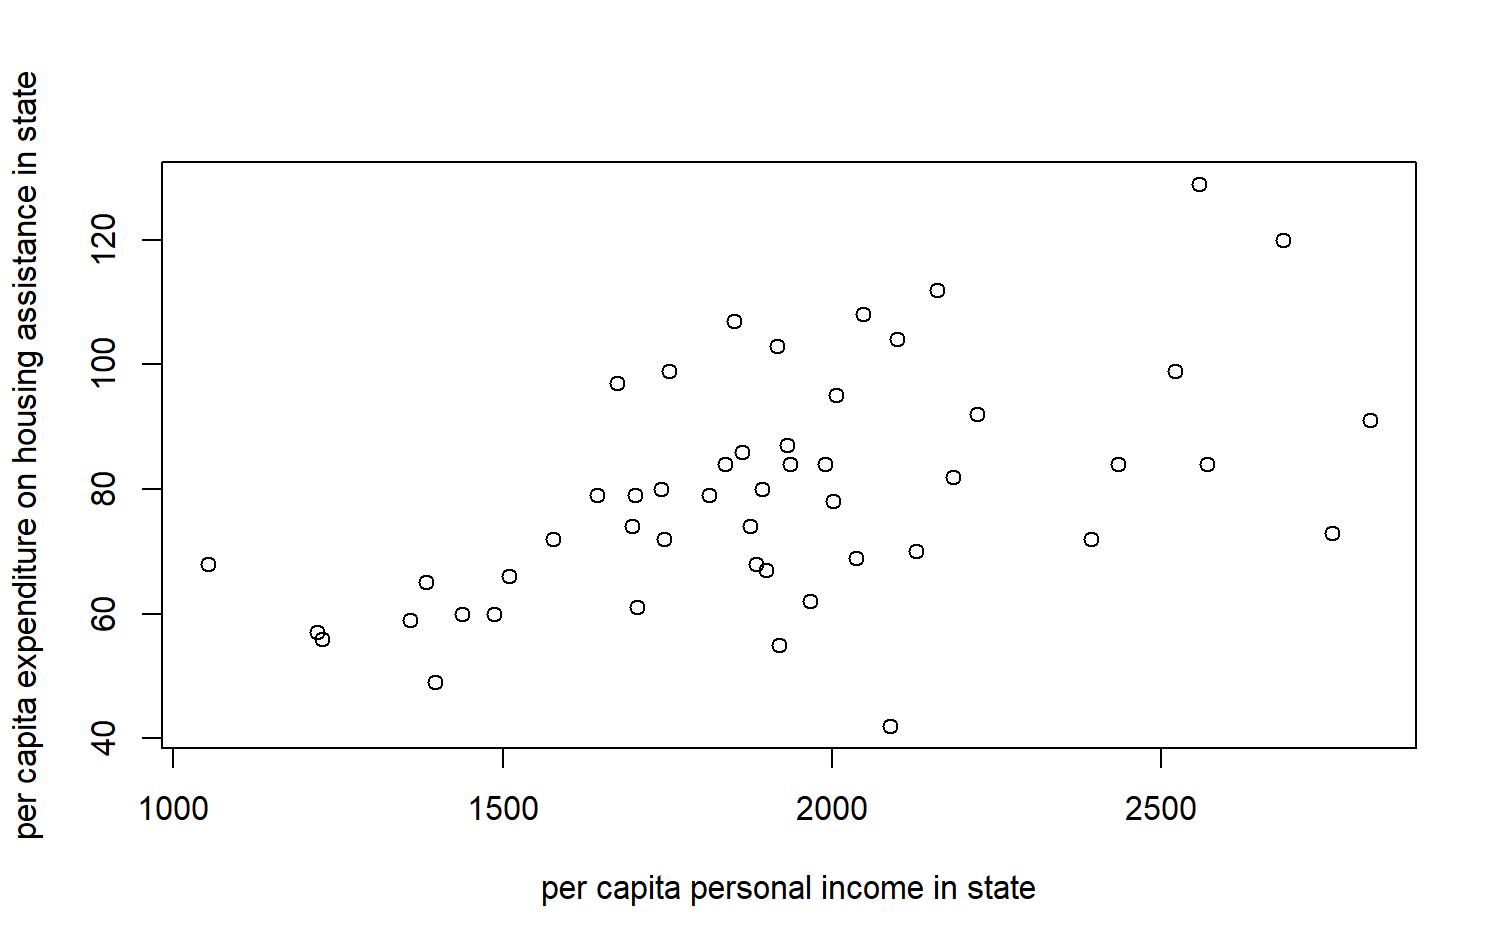
\includegraphics[width=0.8\textwidth]{Figure_1_1.png}
\end{figure}

\begin{itemize}
	\item 
A moderate positive correlation is observable between per capita personal income in state and per capita expenditure on housing assistance in state.
\end{itemize}

\newpage
\lstinputlisting[language=R, firstline=134, lastline=138]{PS01_answers_DMcG.R}
\begin{figure}[H]
	\caption{Scatterplot of relationship between per capita expenditure on housing assistance and financially insecure residents per 100,000 in state}
	\centering
	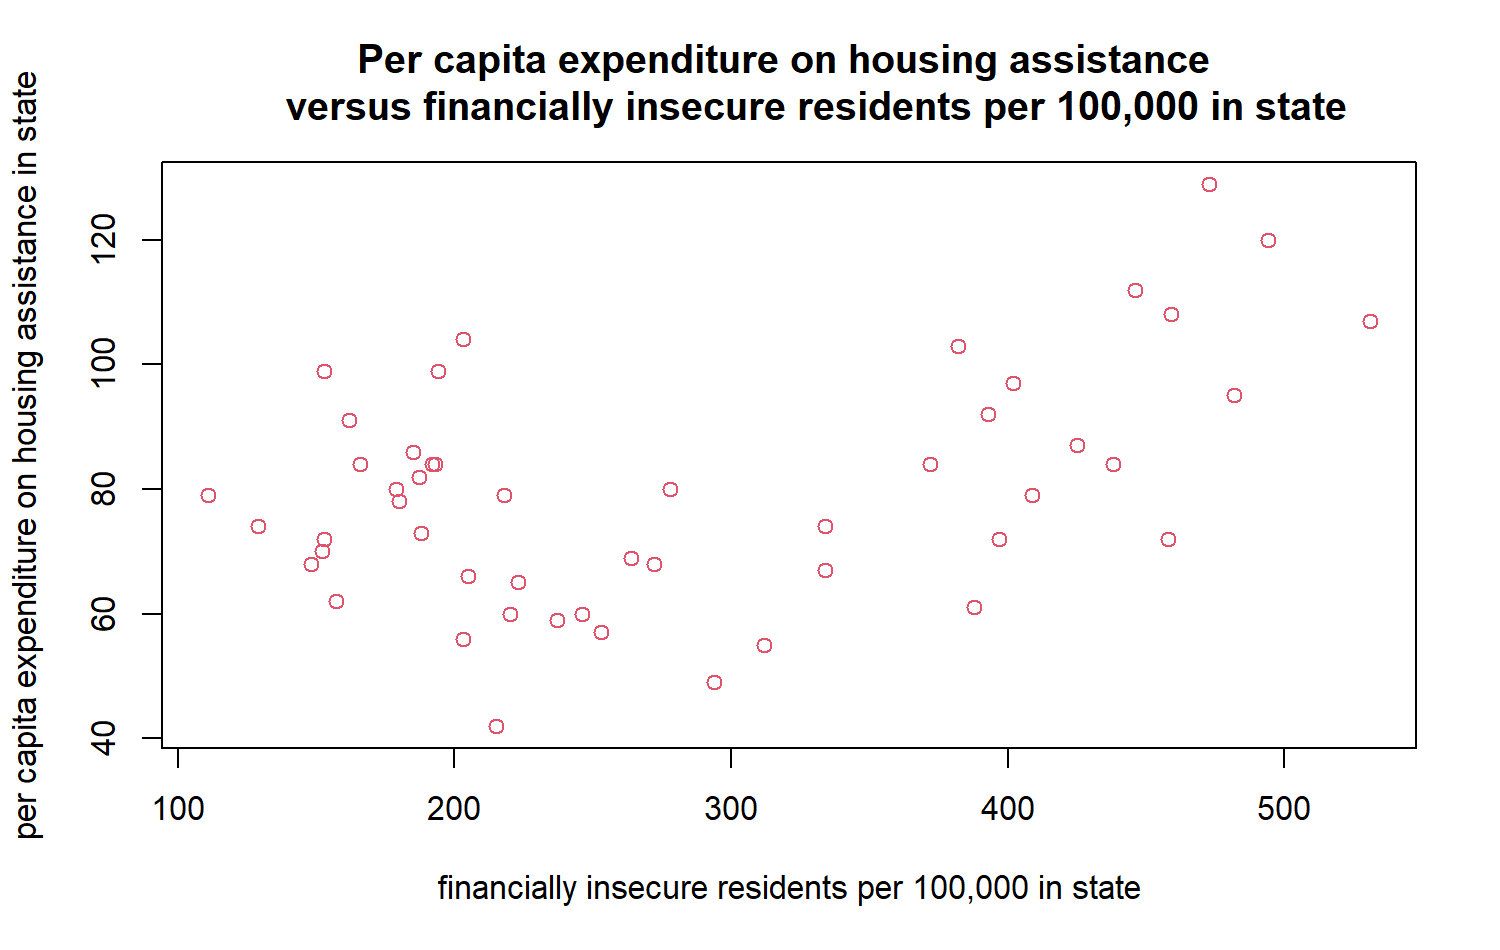
\includegraphics[width=0.8\textwidth]{Figure_1_2.png}
\end{figure}

\begin{itemize}
	\item 
A moderate positive correlation is observable between per capita expenditure on housing assistance and financially insecure residents per 100,000 in the state.
\end{itemize}

\newpage
\lstinputlisting[language=R, firstline=146, lastline=150]{PS01_answers_DMcG.R}
\begin{figure}[H]
	\caption{Scatterplot of relationship between per capita expenditure on housing assistance and people residing in urban areas per 1000 in state}
	\centering
	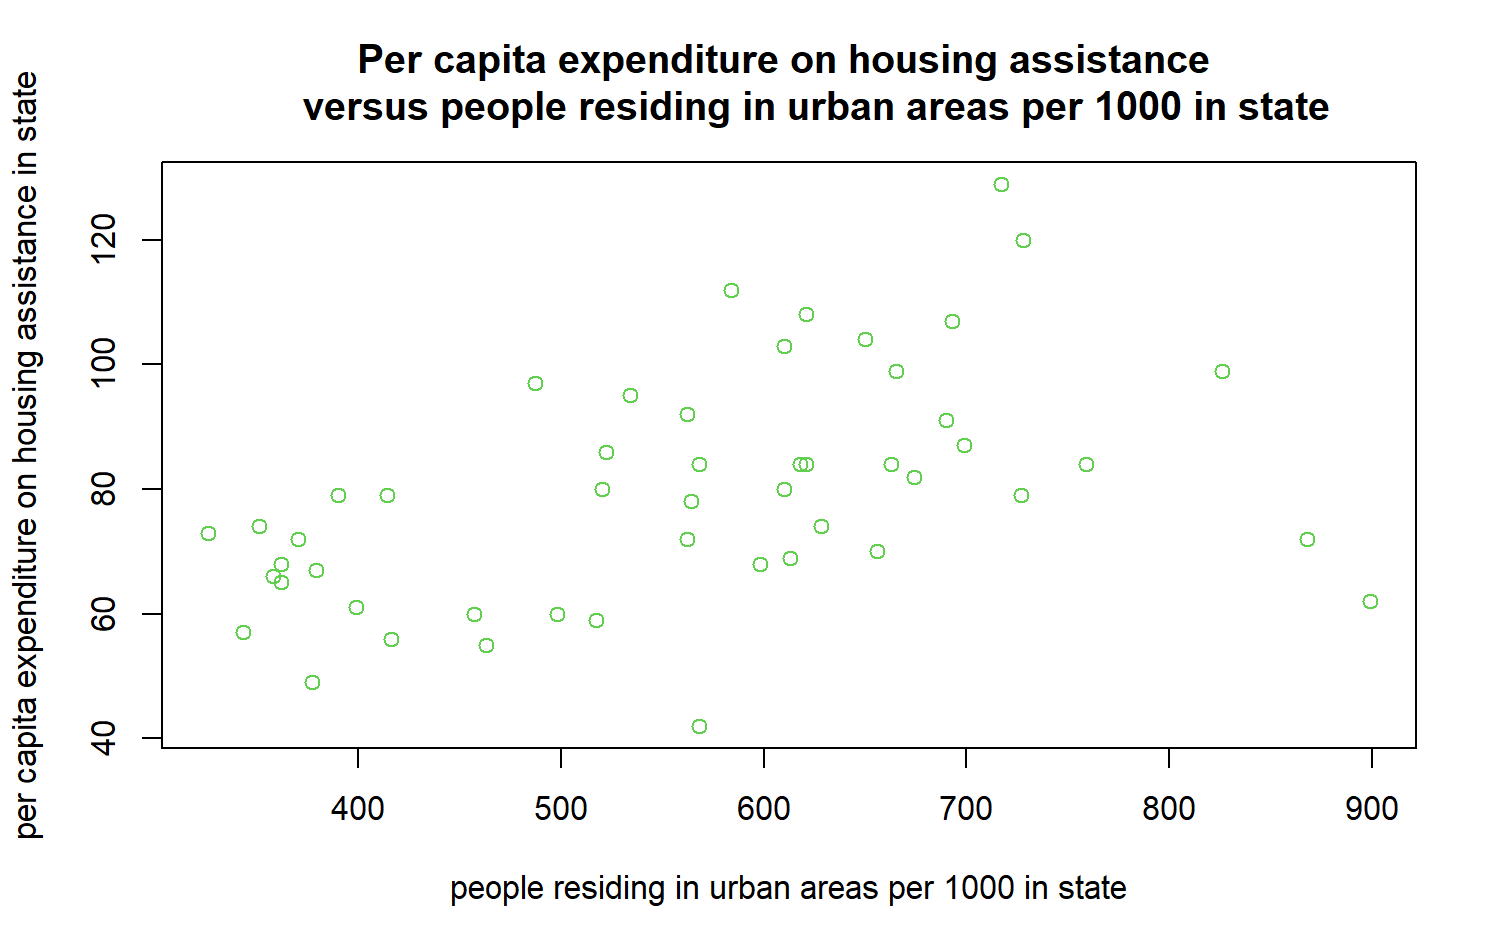
\includegraphics[width=0.8\textwidth]{Figure_1_3.png}
\end{figure}

\begin{itemize}
	\item 
A moderate positive correlation is observable between people residing in urban areas per 1000 in state and per capita expenditure on housing legal assistance in state. 
\end{itemize}

\newpage
\lstinputlisting[language=R, firstline=158, lastline=162]{PS01_answers_DMcG.R}
\begin{figure}[H]
	\caption{Scatterplot of relationship between per capita personal income in state and financially insecure residents per 100,000 in state}
	\centering
	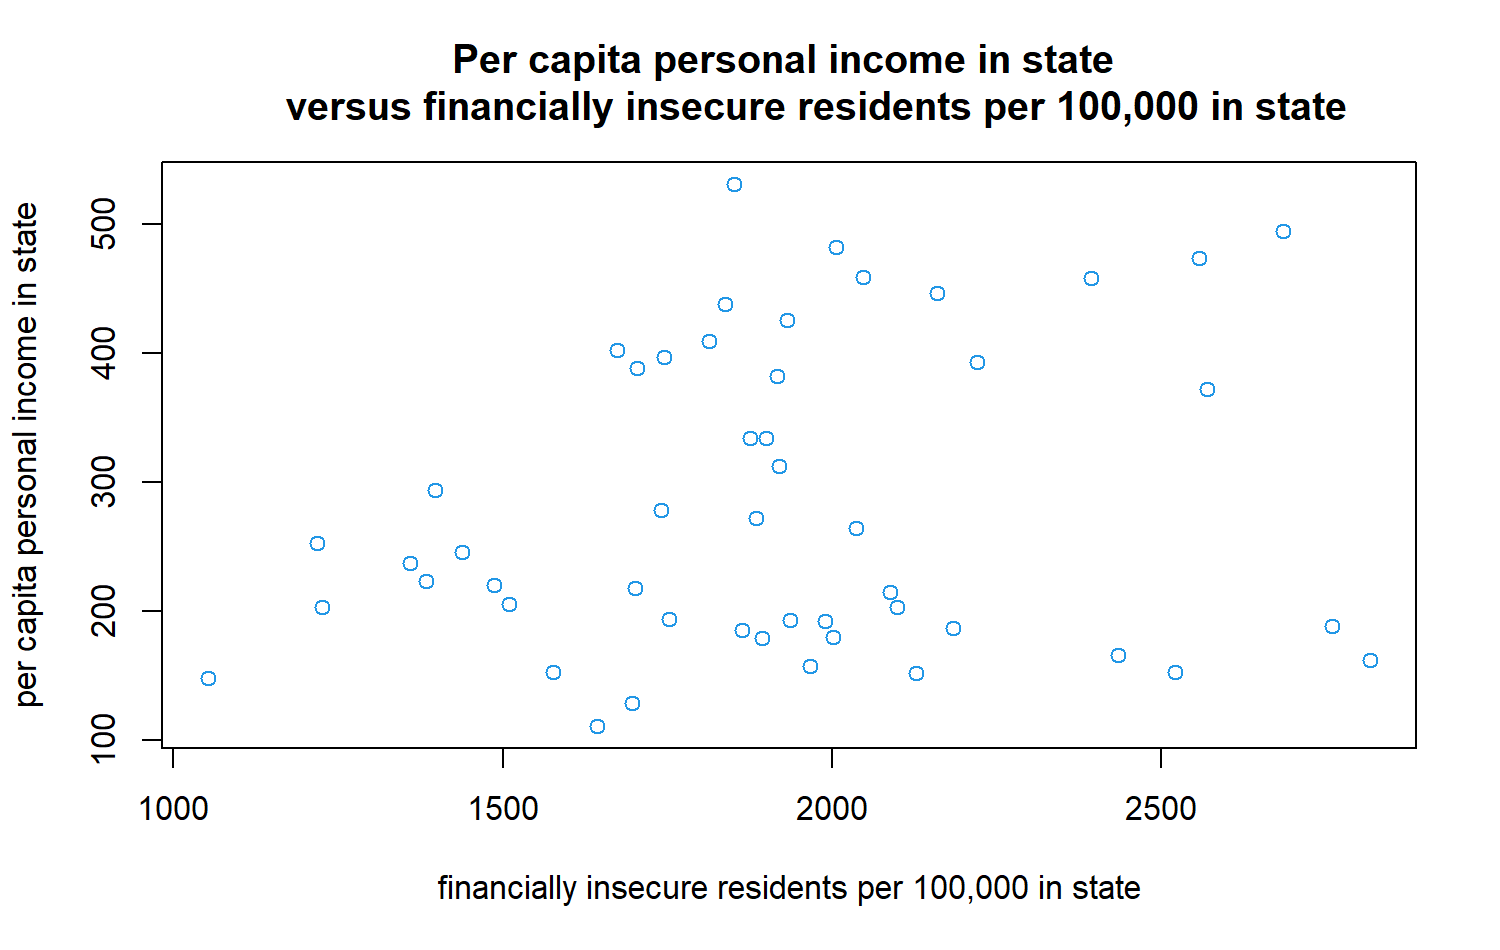
\includegraphics[width=0.8\textwidth]{Figure_1_4.png}
\end{figure}

\begin{itemize}
	\item 
There is no clear linear correlation observable between the per capita personal income in state and financially insecure residents per 100,000 in state. 
\end{itemize}

\newpage
\lstinputlisting[language=R, firstline=169, lastline=173]{PS01_answers_DMcG.R}
\begin{figure}[H]
	\caption{Scatterplot of relationship between per capita personal income in state and people residing in urban areas per 1000 in state}
	\centering
	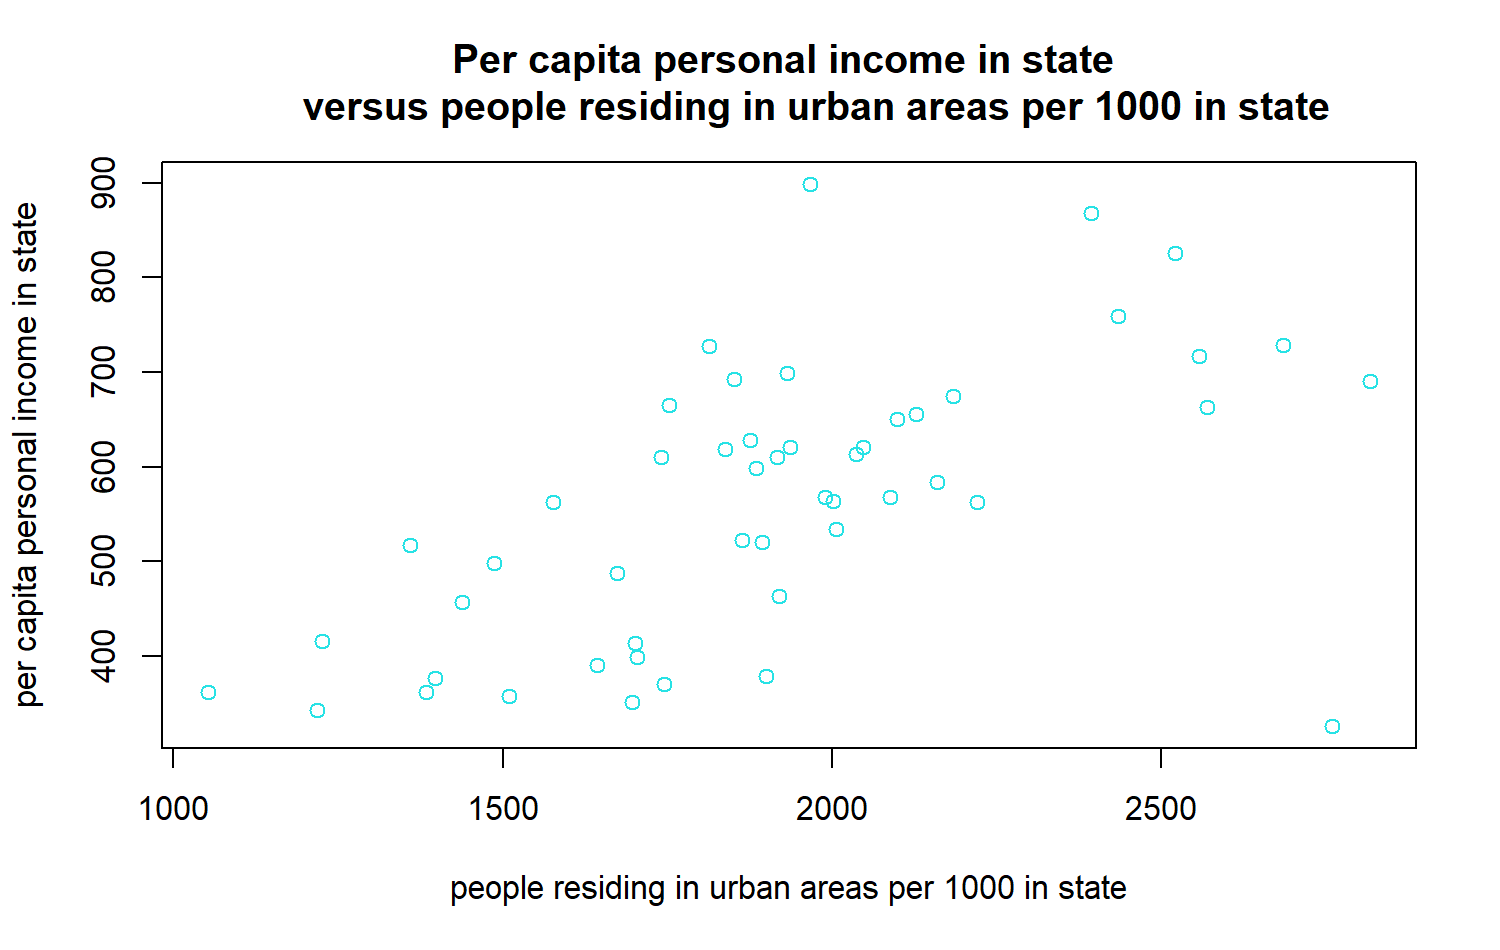
\includegraphics[width=0.8\textwidth]{Figure_1_5.png}
\end{figure}

\begin{itemize}
	\item 
A moderate positive correlation is observable between people residing in urban areas per 1000 in state and per capita personal income in state. 
\end{itemize}

\newpage
\lstinputlisting[language=R, firstline=181, lastline=185]{PS01_answers_DMcG.R}
\begin{figure}[H]
	\caption{Scatterplot of relationship between financially insecure residents per 100,000 in state and people residing in urban areas per 1000 in state}
	\centering
	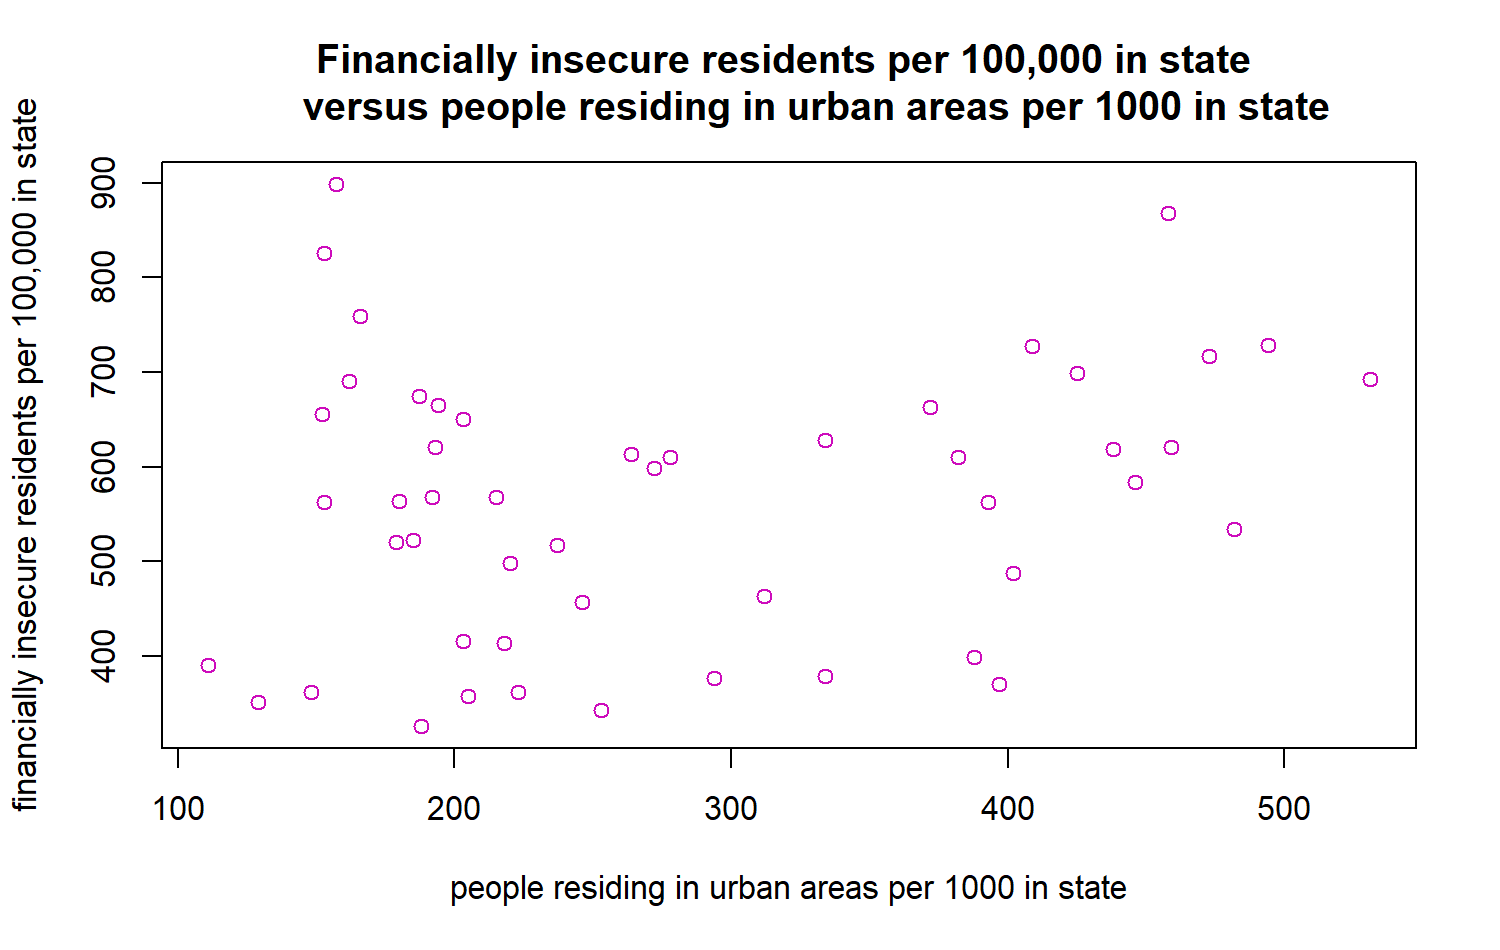
\includegraphics[width=0.8\textwidth]{Figure_1_6.png}
\end{figure}

\begin{itemize}
	\item 
There is no clear linear correlation observable between people residing in urban areas per 1000 in state and financially insecure residents per 100,000 in state.
\end{itemize}

\newpage
\begin{itemize}
\item
Please plot the relationship between \emph{Y} and \emph{Region}? On average, which region has the highest per capita expenditure on housing assistance?
\end{itemize}
\vspace{.5cm}

\lstinputlisting[language=R, firstline=203, lastline=207]{PS01_answers_DMcG.R}
\begin{figure}[H]
	\caption{Boxplot of per capita expenditure on housing assistance per region}
	\centering
	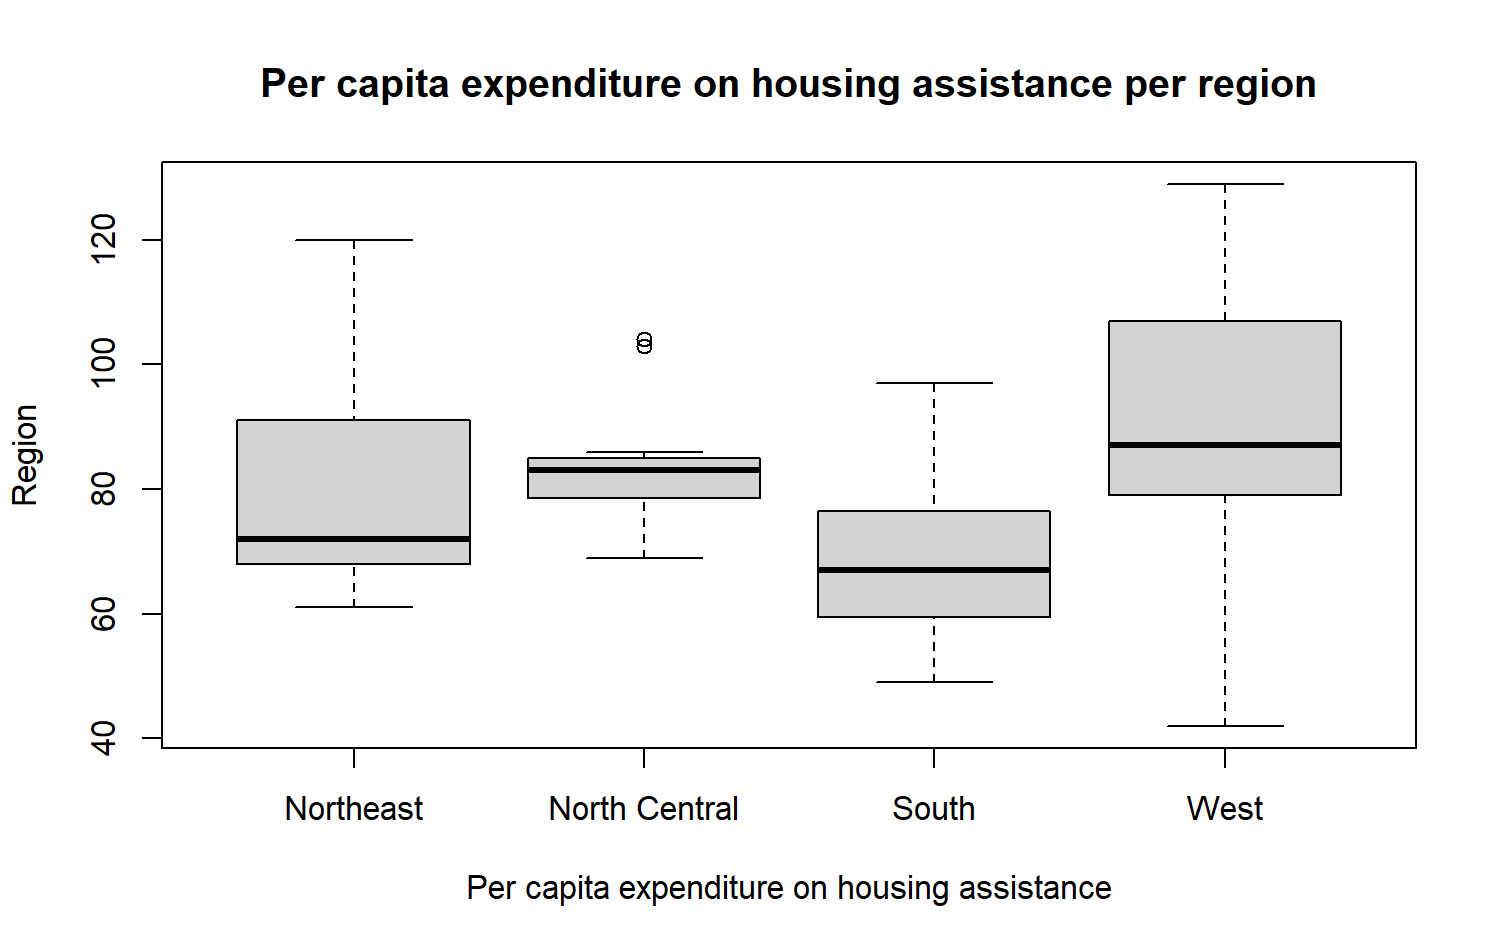
\includegraphics[width=0.8\textwidth]{Figure_2_1.png}
\end{figure}
\vspace{.5cm}

\begin{itemize}
\item 
The box plot visualises the median and interquartile range for per capita expenditure on housing assistance in state. 
\item 
The West Region has the highest median per capita expenditure on housing assistance. There is wide variation in the data for this region, as evidenced by the largest Interquartile Range across Regions. 
\end{itemize}

\newpage
\begin{itemize}
\item
Please plot the relationship between \emph{Y} and \emph{X1}? Describe this graph and the relationship. Reproduce the above graph including one more variable \emph{Region} and display different regions with different types of symbols and colors.
\end{itemize}

\lstinputlisting[language=R, firstline=218, lastline=222]{PS01_answers_DMcG.R}
\begin{figure}[H]
	\caption{Scatterplot of relationship between Per Capita Personal Income and Housing Assistance Expenditure}
	\centering
	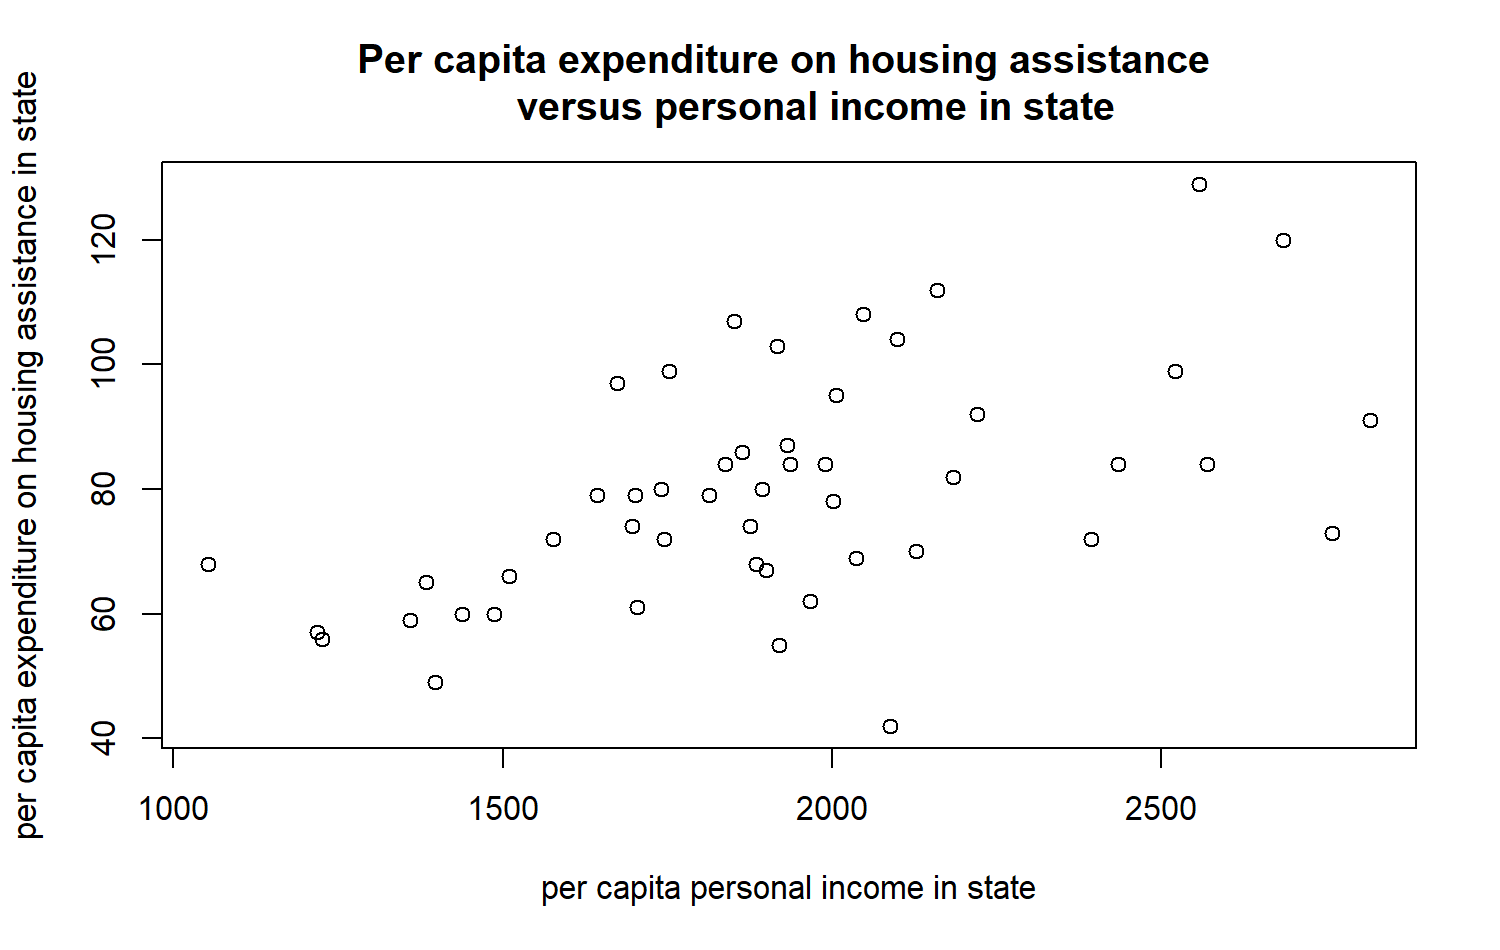
\includegraphics[width=0.8\textwidth]{Figure_2_2.png}
\end{figure}

\begin{itemize}
\item 
A moderate positive correlation is observable between per capita personal income in state and per capita expenditure on housing assistance in state. 
\item 
The data points are relatively spread out, indicating moderate variability in expenditure at similar income levels.  
\item 
There are some outliers in the data, particularly at higher end of per capita personal income in state. 
\end{itemize}

\newpage
\lstinputlisting[language=R, firstline=233, lastline=246]{PS01_answers_DMcG.R}
\begin{figure}[H]
	\caption{Scatterplot of relationship between Per Capita Personal Income and Housing Assistance Expenditure by Region}
	\centering
	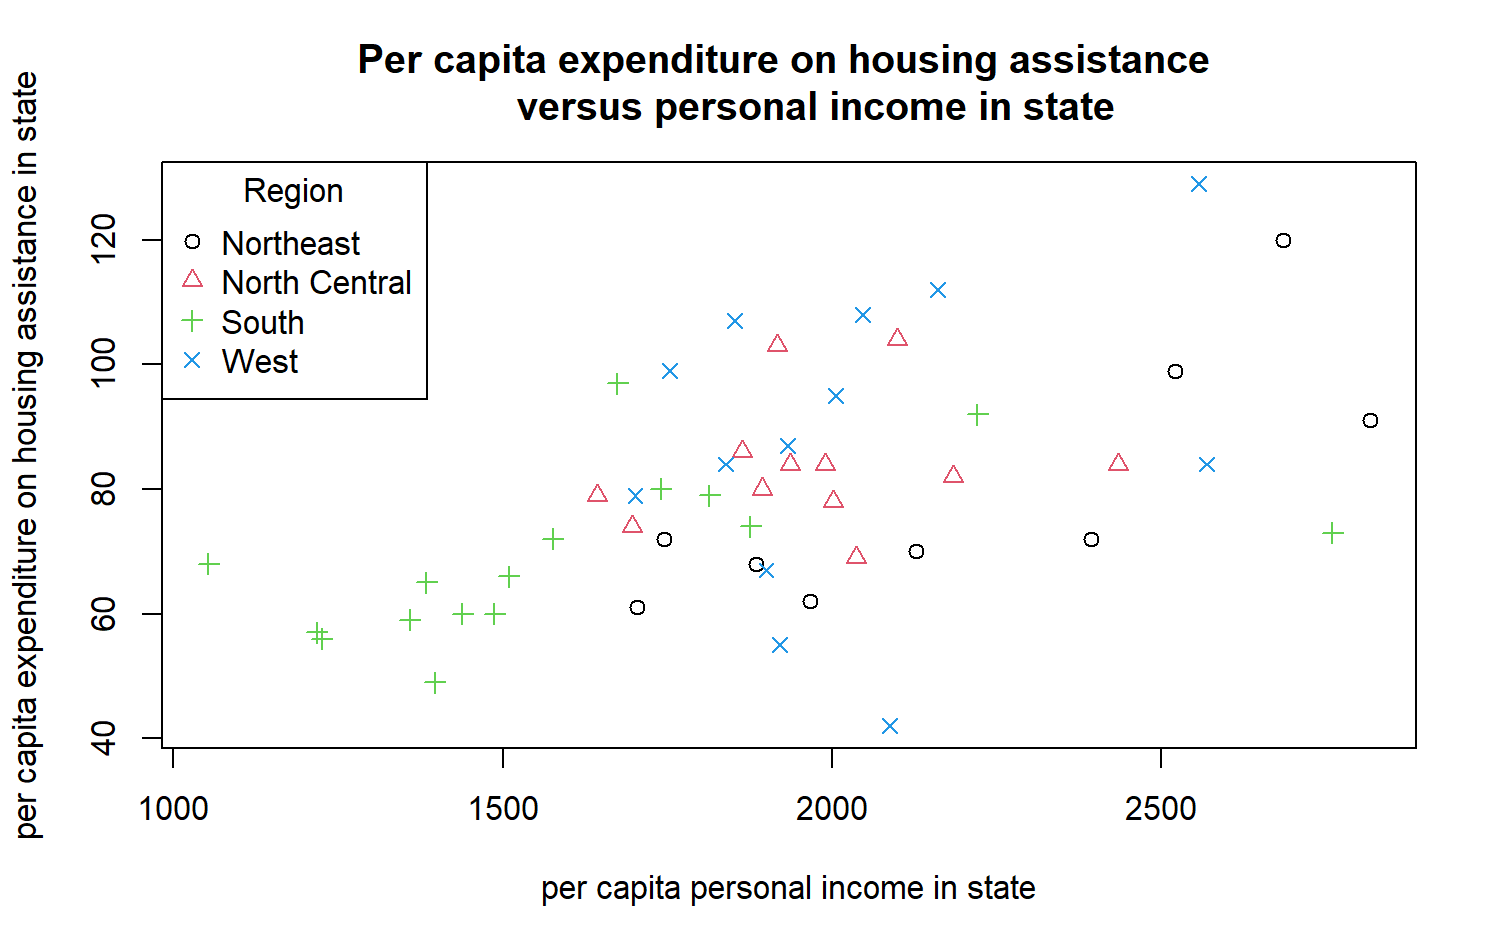
\includegraphics[width=0.8\textwidth]{Figure_2_3.png}
\end{figure}
\begin{itemize}
\item 
Overall, there is a general upward trend, indicating that states with higher per capita income tend to spend more on housing assistance per capita.
\item 
The Northeast and West Regions show that higher per capita income states spend more per capita on housing assistance.
\item
North Central states show moderate expenditures on housing assistance at moderate income levels, with some variability.
\item 
Southern States tend to have lower per capita income in state and lower per capita expenditure on housing assistance in state. 
\end{itemize}

\end{document}
